\section{Extension to Higher Dimensions}\label{sec:mud-higher-dimensions}
We now show that when the dimension of $\pspace$ is higher, the benefit from maximizing the dimension of the QoI map is even more considerable than what we observed in the two-dimensional cases, as long as we aggregate data into components of the QoI map in a purposeful manner.
In the first example, we demonstrate the impact of increasing the volume of the parameter space while fixing all other attributes of the inverse problem.
In the second example, we illustrate how we could utilize the solution to the SIP for the two-dimensional case from \ref{subsec:pde-example} to improve the MUD estimate in five dimensions.

\subsection{A SIP with a Naive Initial Density}
Consider a naive implementation in five dimensions, where the same prior knowledge on the bounds of $g$ inform the choice of a parameter space.
Suppose $\pspace$ is given by $[-4, 0]^5$, induced by five regularly-spaced knot points in the interior of $x_2 \in (0,1)$ for which a uniform density is assumed in each component.
In Figure~\ref{fig:pde-highd-initial-5d}, we show what one-thousand such initial functions look like, and note that many of them appear to exhibit fluctuating behavior which may require a finer mesh than the one being used to solve the problem ($36\times36$), in order to reduce numerical errors.
This choice of initial density induces a lot of ``conceptual'' noise into the SIP, since ``common sense'' from a modeler's perspective could rule out functions which zig-zag excessively.

\begin{figure}
\centering
  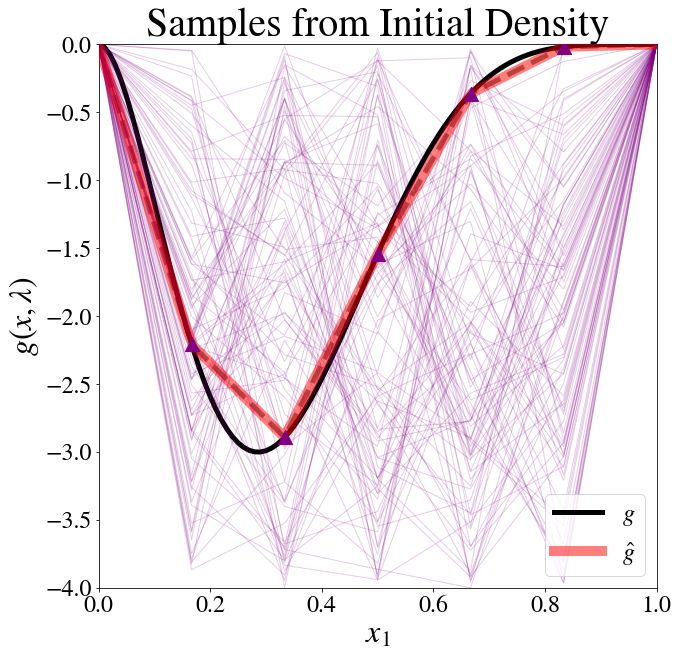
\includegraphics[width=0.475\linewidth]{figures/pde-highd/pde-highd_init_D5.png}
\caption{
One thousand initial parameter samples (our model evaluation ``bugdet'') were used to estimate $g$, constructed by taking independent uniform samples from $[-4, 0]$ for each direction are shown in purple.
}
\label{fig:pde-highd-initial-5d}
\end{figure}

We solve the SIP for both scalar-- and vector--valued QoI maps.
The latter is constructed with horizontal bands\---which correspond to the partitioning of $\Omega$ into components of the QoI map\---shown in the left of Figure \ref{fig:pde-highd-5d-example}.
We refer to this map as $\qoi_\text{5D}$, and $\qoi_\text{1D}$ will again represent the scalar--valued map.
In the right half of Figure~\ref{fig:pde-highd-5d-example}, the MUD solutions for $\qoi_\text{5D}$ and $\qoi_\text{1D}$ are shown in parameter space for a representative SIP.
The scalar-valued MUD misidentifies the location of $g$'s minimum value, but the vector-valued QoI is able to resolve the general qualitative behavior.

\begin{figure}
\centering
  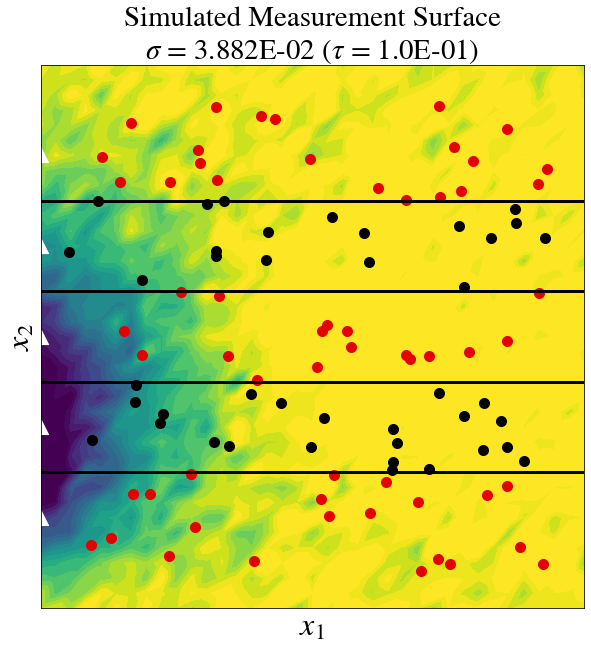
\includegraphics[width=0.45\linewidth]{figures/pde-highd/pde-highd_sensors_D5}
  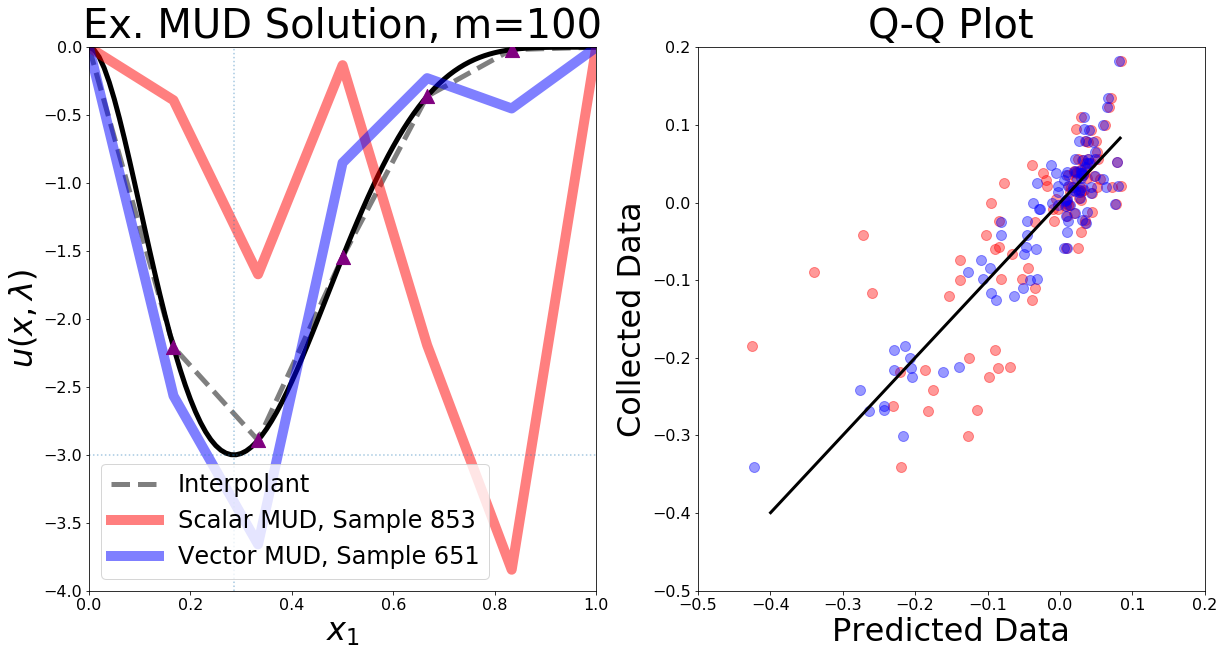
\includegraphics[width=0.45\linewidth]{figures/pde-highd/pde-highd_comp_exmud_D5_m100}
\caption{
(Left): Layout for 5-D vector--valued map and comparison of the two MUD solutions in parameter space.
(Right): Example MUD solutions for $\qoi_\text{5D}$ and $\qoi_\text{1D}$.
}
\label{fig:pde-highd-5d-example}
\end{figure}

In Figure~\ref{fig:pde-highd-5d-mud} we plot the results from twenty repeated trials (perturbations of noise) when using all hundred measurements, and observe the same difference in going from scalar-- to vector--valued solutions for the five--dimensional example that we saw in two dimensions with \ref{fig:pde-highd-2d-vector-mud}.
In the left half of Figure~\ref{fig:pde-highd-5d-mud}, the scalar-valued QoI is unable to differentiate between resolving residual discrepancies in different locations in $\Omega$.
By contrast, the vector-valued QoI shown to the right is constructed with respect to the flow of information in the system, and so many more of the twenty trials land closer to the true minimum value of $g$.
The solutions for the vector-valued approach instead explore the available knots (at $x_2=1/6$ and $1/3$), nearest the actual minimum value of $2/7$ instead, a much more valuable area of $\Lambda$ to explore.

\begin{figure}
\centering
  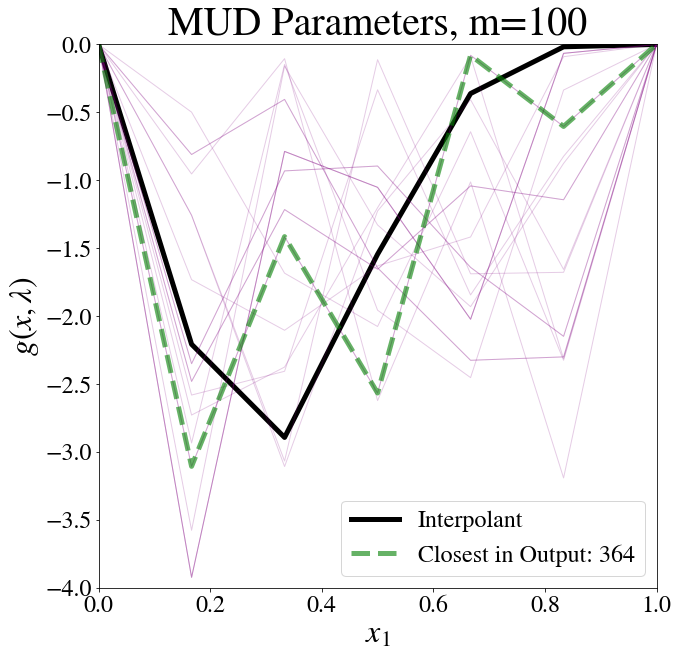
\includegraphics[width=0.45\linewidth]{figures/pde-highd/pde-highd_pair_D5-1_m100}
  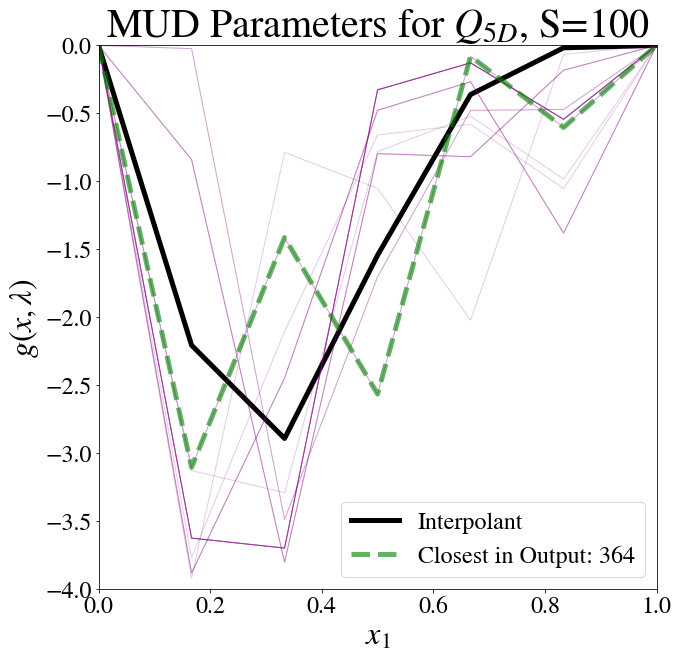
\includegraphics[width=0.45\linewidth]{figures/pde-highd/pde-highd_pair_D5-5_m100}
\caption{ SIP solutions using $\qoi_\text{5D}$ and $\qoi_\text{1D}$ for twenty realizations of noise polluting the hundred measurements used to construct the map.
(Left): Scalar-valued solutions.
(Right): Vector-valued solutions.
}
\label{fig:pde-highd-5d-mud}
\end{figure}


Recall from \ref{subsec:pde-example} that we previously solved a two-dimensional version of this problem.
We leverage the effort involved in solving this first problem in order to better refine the approximation of $g$ in \ref{sec:mud-pde-sequence} below.
By using the former SIP solution results to define a much smaller region of $\pspace$ to explore, the results from the second SIP can improve considerably.
